\section{Verification using Functional Probabilistic Invariants}
\begin{frame}<1-5>[label=algsplit]
\frametitle{Another slide with the algorithm}
\begin{algorithmic}
  \State $\chi \gets \{\}, p \gets 1, n = \ceil*{\frac{12}{\varepsilon^2} \ln{(\frac{\only<6>{3}\only<1-5>{6}l}{\delta})} }$
  \For{$i \gets 1$ to $l$}
    \State $b \getsr \Ber(p)$
    \If{$b$}
      \State $\chi \gets \chi \cup \{a_i\}$
    \Else
      \State $\chi \gets \chi - \{a_i\}$
    \EndIf
    \If{$|\chi| = n$}
      \State $\chi \getsr \only<1-5>{\mathrm{subsample}}\only<6>{\mathrm{subsample'}}(\chi)$
      \State $p \gets \frac{p}{2}$
    \EndIf
    \If{$|\chi| = n$}
      \Return $\bot$
    \EndIf
  \EndFor
  \State \Return $\frac{|\chi|}{p}$
\end{algorithmic}

\tikz[overlay, shift=(current page.north west)]{
\begin{scope}[x={(current page.north east)},y={(current page.south west)}]

\only<2->{
        \fill[blue!50, opacity=0.5] (0.07,0.4) rectangle (0.7,0.67);
        \node [anchor=west] at (0.45,0.535) {Step 1};
}
\only<3->{
        \fill[red!50, opacity=0.5] (0.07,0.675) rectangle (0.7,0.845);
        \node [anchor=west] at (0.45,0.76) {Step 2};
}
\only<4->{
        \draw[thick, decorate, decoration={snake,amplitude=0.6pt}] (0.072,0.87) -- (0.42, 0.87);
}
\only<6>{
       \fill[white] (0.07,0.846) rectangle (0.7,0.895);
}
\only<5->{
  \fill[green!50, opacity=0.5] (0.03, 0.895) rectangle (0.7, 0.97);
   \node [anchor=west] at (0.45,0.932) {Estimate};
}
\end{scope}
}
\end{frame}

\begin{frame}
\frametitle{Giry Monad}
We can represent randomized algorithms using the Giry monad:
\begin{itemize}
\item Primitive random operations, e.g., $\Ber(p)$
\item Return operation $\mathrm{return} \, x$
\item Sequential compositon $m \mbind f$
\end{itemize}
\pause
\begin{block}{Fact}
For an event $E$: 
\begin{eqnarray*}
\prob_{m \mbind f}( E )  & = & \int_{m} P_{f(x)} (E) \, dx \onslide<3->{= \sum_x P_{f(x)} (E) P_m({x})} \\
\onslide<4->{\expect_{m \mbind f}[ g ]  & = & \int_{m} \expect_{f(x)} [g] \, dx}
\end{eqnarray*}
\end{block}
\end{frame}

\againframe<5>{algsplit}

\begin{frame}
\frametitle{Our algorithm in monadic notation}
\newcommand{\stepone}{\textcolor{blue}{\mathrm{step}_1}}
\newcommand{\steptwo}{\textcolor{red}{\mathrm{step}_2}}
\newcommand{\estimate}{\textcolor{green}{\mathrm{estimate}}}
\begin{eqnarray*}
  \mathrm{init} & \mbind & \stepone a_1 \mbind \steptwo \mbind \stepone a_2 \mbind \steptwo \cdots \\
  & \mbind & \stepone a_l \mbind \steptwo \mbind \estimate \\
  \mathrm{init} & = & \mathrm{return} \, (1, \emptyset)
\end{eqnarray*}
\pause
Example invariant:
\[
\expect \left[ \frac{\indicat(s \in \chi)}{p} \right]= 1
\]
for all $s$ that are present in the stream.
\end{frame}

\begin{frame}
\frametitle{Verifying the invariant: Induction step for Step 2}
\begin{block}{Assumption}
$\expect_m \left[ \frac{\indicat(s \in \chi)}{p} \right] = 1$
\end{block}
\begin{block}{Goal}
$ L := \expect_{m \mbind \mathrm{step}_2} \left[ \frac{\indicat(s \in \chi)}{p} \right]= 1$
\end{block}
\[
L =
\only<1>{\expect_{m \mbind \mathrm{step}_2} \left[ \frac{\indicat(s \in \chi)}{p} \right]}
\only<2>{\integral{m}
      {\left(\ift{|\chi|=n}{\integral{\mathrm{subs.}(\chi)}{\frac{\indicat(s \in \tau)}{p/2}}{\tau}}{\frac{\indicat(s \in \chi)}{p}} \right)}
      {\sigma}}
\only<3>{\integral{m}
      {\left(\ift{|\chi|=n}{\frac{2}{p}\integral{\mathrm{subs.}(\chi)}{\indicat(s \in \tau)}{\tau}}{\frac{\indicat(s \in \chi)}{p}} \right)}
      {\sigma}}
\only<4>{\integral{m}
      {\left(\ift{|\chi|=n}{\frac{2}{p}\frac{\indicat(s \in \chi)}{2}}{\frac{\indicat(s \in \chi)}{p}} \right)}
      {\sigma}}
\only<5>{\integral{m}
      {\left(\ift{|\chi|=n}{\frac{\indicat(s \in \chi)}{p}}{\frac{\indicat(s \in \chi)}{p}} \right)}
      {\sigma}}
\only<6>{\integral{m}
      {\frac{\indicat(s \in \chi)}{p} }
      {\sigma}}
\only<7>{1}
\]
\end{frame}

\begin{frame}[label=observations]
\frametitle{Observations}
\begin{itemize}
\item Expected result is the count of distinct elements.
\only<2->{\item We want to establish concentration}
\only<4->{\item Can extend the above recursive analysis to more complex expressions: }
\only<5>{
\[
  \expect \left[ h \left( \frac{\indicat(s \in \chi)}{p} \right)\right] \leq h(1)
\]
for every non-negative concave function $h$ and stream elements $s$.}
\only<6->{
\[
  \expect \left[ \prod_{s \in S}  h \left( \frac{\indicat(s \in \chi)}{p} \right)\right] \leq h(1)^{|S|}
\]
for every non-negative concave function $h$ and subset of stream elements $S$.}
\only<7->{\item $\Rightarrow$\only<8->{*} Approximation Guarantee
\[
  \prob\left(|X - |A|| \geq \varepsilon |A| \right) \leq \delta 
\]
\only<8->{\item More details in the paper.}
}
\end{itemize}
\only<3>{
\begin{figure}
\centering
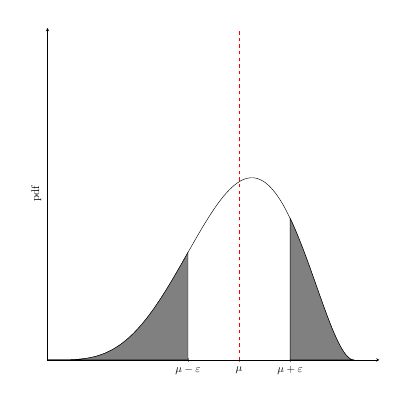
\begin{tikzpicture}[scale=0.4]
\begin{axis}[
    xmin=0, xmax = 6.5,
    ymin=0, ymax=0.7,
    axis lines = left,
    xlabel = {},
    xtick={2.75,3.75,4.75},
    xticklabels={$\mu-\varepsilon$,$\mu$,$\mu+\varepsilon$},
    ytick=\empty,
    ylabel = {pdf},
    height = \textwidth,
    width = \textwidth,
]
\addplot [
    domain=0:6, 
    samples=1000, 
]{max(0,35/2*(x/6)^4*(1-x/6)^2)};
\addplot [
    domain=4.75:6, 
    samples=1000, 
    fill=gray,
]{max(0,35/2*(x/6)^4*(1-x/6)^2)} \closedcycle;
\addplot [
    domain=0:2.75, 
    samples=1000, 
    fill=gray,
]{max(0,35/2*(x/6)^4*(1-x/6)^2)} \closedcycle;
\draw[color=red, dashed] (axis cs:3.75, 0) -- (axis cs:3.75, 0.7);
\end{axis}
\end{tikzpicture}
\begin{tikzpicture}[scale=0.4]
\begin{axis}[
    xmin=0, xmax = 6.5,
    ymin=0, ymax=0.7,
    axis lines = left,
    xlabel = {},
    xtick={2.75,3.75,4.75},
    xticklabels={$\mu-\varepsilon$,$\mu$,$\mu+\varepsilon$},
    ytick=\empty,
    ylabel = {pdf},
    height = \textwidth,
    width = \textwidth,
]
\addplot [
    domain=0:6, 
    samples=1000, 
]{0.65*exp(-(2*(x-3.75))^2)};
\addplot [
    domain=4.75:6, 
    samples=1000, 
    fill=gray,
]{0.65*exp(-(2*(x-3.75))^2)} \closedcycle;
\addplot [
    domain=0:2.75, 
    samples=1000, 
    fill=gray,
]{0.65*exp(-(2*(x-3.75))^2)} \closedcycle;
\draw[color=red, dashed] (axis cs:3.75, 0) -- (axis cs:3.75, 0.7);
\end{axis}
\end{tikzpicture}
\end{figure}
}
\end{frame}

\begin{frame}
\frametitle{Observations II}
\begin{itemize}
\item The new proof is much shorter than the original proof (1003 lines vs. 2634 lines.)
\item<2-> \emph{As far as we can tell,} this technique is new.
\item<3-> The new proof opens up the design-space of the algorithm.
\item<4,6-> \only<4>{For example we can select the subsampling ratio dynamically.}\only<6->{More interestingly: It is possible to use a different subsampling operation.}
\item<7-> Select a random $nf$-subset (where $\frac{1}{2} \leq f < 1$, $nf \in \mathbb Z$).
\item<8-> $\Rightarrow$ Unbiased algorithm
\end{itemize}
\end{frame}
\againframe<5-6>{algsplit}

